

\begin{frame}{AlphaGo}
    \begin{center}

        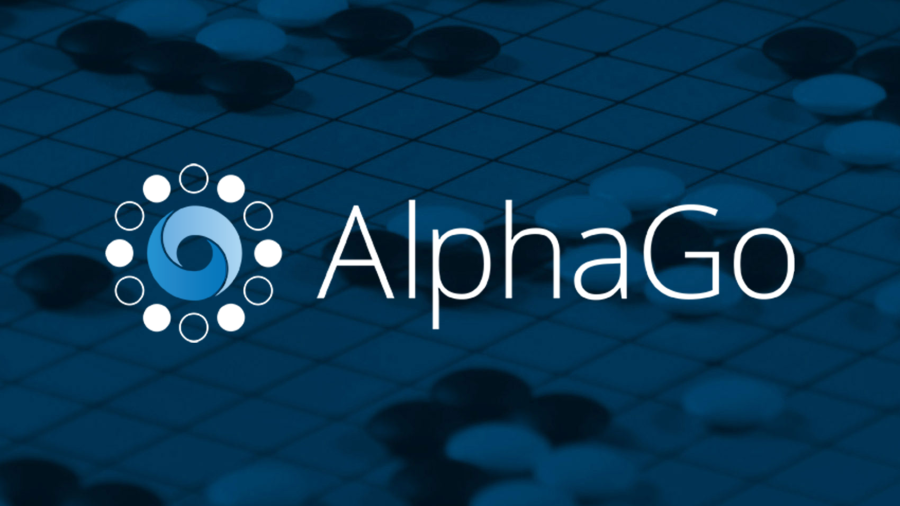
\includegraphics[width=5cm]{ressources/AlphaGo/AlphaGoLogo}
    \end{center}
    \begin{block}{}
        \begin{itemize}
            \item Développé par Google DeepMind
            \item En mars 2016 \textbf{AlphaGo} a battu Lee Sedol, l'un des meilleurs joueurs de Go
        \end{itemize}
    \end{block}
    \begin{exampleblock}{\textbf{Technologies utilisées:}}
        \begin{itemize}
            \item Apprentissage par renforcement
            \item Réseaux de neurones profonds
            \item Monte Carlo Tree Search
        \end{itemize}
    \end{exampleblock}
\end{frame}



\begin{frame}{AlphaGo}{Composants}
    \begin{center}
        \textbf{Composants}
    \end{center}
    \begin{columns}[t]
        \begin{column}{.3\textwidth}
            \begin{block}{Policy network}
                Réseau neuronal qui renvoie une \textbf{distribution de probabilité} sur le coups possibles.
            \end{block}
        \end{column}
        \begin{column}{.3\textwidth}
            \begin{block}{Value Network}
                Réseau neuronal chargé d'estimer la \textbf{valeur} d'une position.            \end{block}
        \end{column}
        \begin{column}{.3\textwidth}
            \begin{block}{Fast Rollout policy}
                Politique plus simple que les autres qui permet une \textbf{simulation rapide} du reste de la partie.
            \end{block}
        \end{column}
    \end{columns}
\end{frame}

\begin{frame}{AlphaGo}{Entraînement des réseaux neuronales}
    \begin{center}
        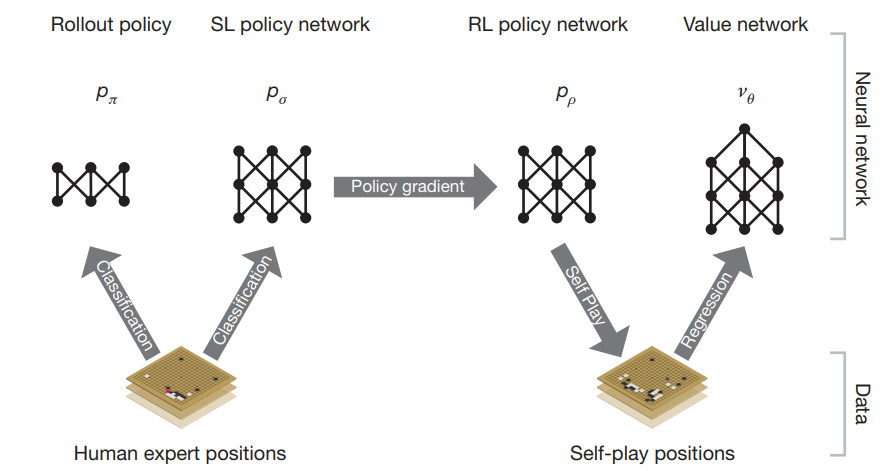
\includegraphics[width=7cm]{ressources/AlphaGo/Entrainement}
        \begin{columns}[t]
            \begin{column}{.4\textwidth}
                \begin{block}{Avec un modèle}
                    Entraînement d'un réseau \textbf{supervisé} (SL).
                \end{block}
            \end{column}
            \begin{column}{.4\textwidth}
                \begin{block}{Self-play}
                    Apprentissage par renforcement à partir du SL en jouant des parties \textbf{contre soi-même}.
                \end{block}
            \end{column}
        \end{columns}

    \end{center}
\end{frame}


\begin{frame}{AlphaGo}{Apprentissage avec un modèle (SL)}
    \begin{center}

        \begin{block}{Objectif}
            Modèle qui prédit, à partir d'un état $s$, l'action $a$ qu'un joueur professionnel aurait fait.
        \end{block}
        \vspace{1cm}
        \begin{block}{Solution}
            Réseau neuronal convolutif avec 13 couches.
            Entraînement initial \textbf{supervisé} à partir de parties jouées par des professionnels (30 million de positions différentes).
        \end{block}
    \end{center}
\end{frame}

\begin{frame}{AlphaGo}{Apprentissage avec un modèle (SL)}
    \begin{block}{Resultat}
        Politique $p_\sigma$, avec $\sigma$ les paramètres (les poids) du réseau.
        Temps d'évaluation de l'ordre de \textbf{3 ms} avec une précision de \textbf{57.0\%}.
    \end{block}
    \begin{center}
        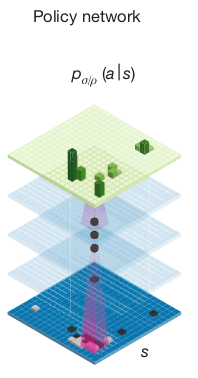
\includegraphics[scale=0.4]{ressources/AlphaGo/Policy_Network}
    \end{center}
\end{frame}

\begin{frame}{AlphaGo}{Self-play}
    \begin{block}{Objectif}
        \begin{center}
            Trouver une politique \textbf{meilleure} que $p_\sigma$.
        \end{center}
    \end{block}

    \begin{block}{Solution}
        \begin{itemize}
            \item Entraînement par renforcement en jouant des parties contre \textbf{soi-même}.
            \item Système de recompense simple : +1 si victoire et -1 si défaite.
            \item Structure \textbf{égale à celle du SL}, avec une politique $p_\rho$, avec des poids initiales égaux à $\sigma$.
            \item Parties entre la version actuelle de l'agent et une \textbf{version antérieure aléatoire}.
            \item Taux de réussite contre le SL : \textbf{80\%}.
        \end{itemize}
    \end{block}
\end{frame}


\begin{frame}{AlphaGo}{Value network}
    La \textbf{value network} nous permet d'estimer la \textbf{valeur} d'une position.
    \begin{block}{Modèle théorique}
        On définit $v^p$ comme la fonction qui prédit le résultat de la partie en partant de la position $s$ suivant la politique $p$.$$v^p(s) = \mathbb{E}[z_t|s_t=s, a_{t,\dots,T}\sim p]$$
        L'idéal est de trouver $v^*$, la fonction de valeur optimale, mais c'est impossible.
        On décide d'utiliser la meilleur politique qu'on connaît: $p_\rho$, ainsi on peut \textbf{approximer} la valeur de $v^*$. $$v_\theta(s) \approx v^{p_\rho}(s) \approx v^*(s)$$
    \end{block}
\end{frame}

\begin{frame}{AlphaGo}{Value network}
    \begin{block}{Solution}
        \begin{itemize}
            \item Utiliser un réseau de neurones profond.
            \item Sa structure est la même que celle du RL mais avec \textbf{une seule sortie} et il est entraîné sur la RL.
        \end{itemize}
    \end{block}
    \begin{center}
        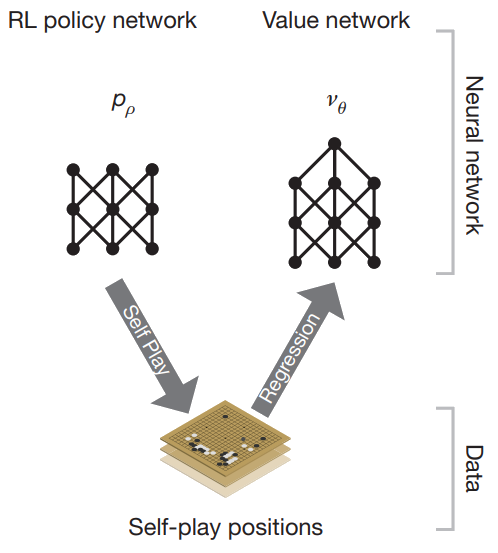
\includegraphics[width=5cm, height=5.2cm]{ressources/AlphaGo/RL_and_VN}
    \end{center}
\end{frame}

\begin{frame}{AlphaGo}{Fast rollout policy}
    \begin{block}{Objectif}
        \begin{center}
            Politique \textbf{rapide} qui permet de \textbf{simuler} le reste de la partie.
        \end{center}
    \end{block}
    \begin{block}{Solution}
        \begin{itemize}
            \item
            \item Entraîné avec le même modèle que le SL.
            \item Architecture beaucoup plus simple.
            \item Politique $p_\pi$.
            \item Précision de \textbf{24.2\%}.
            \item Temps d'évaluation de \textbf{2} $\boldsymbol{\mu s}$.
        \end{itemize}
    \end{block}
\end{frame}


\begin{frame}{AlphaGo}{MCTS}
    \begin{center}
        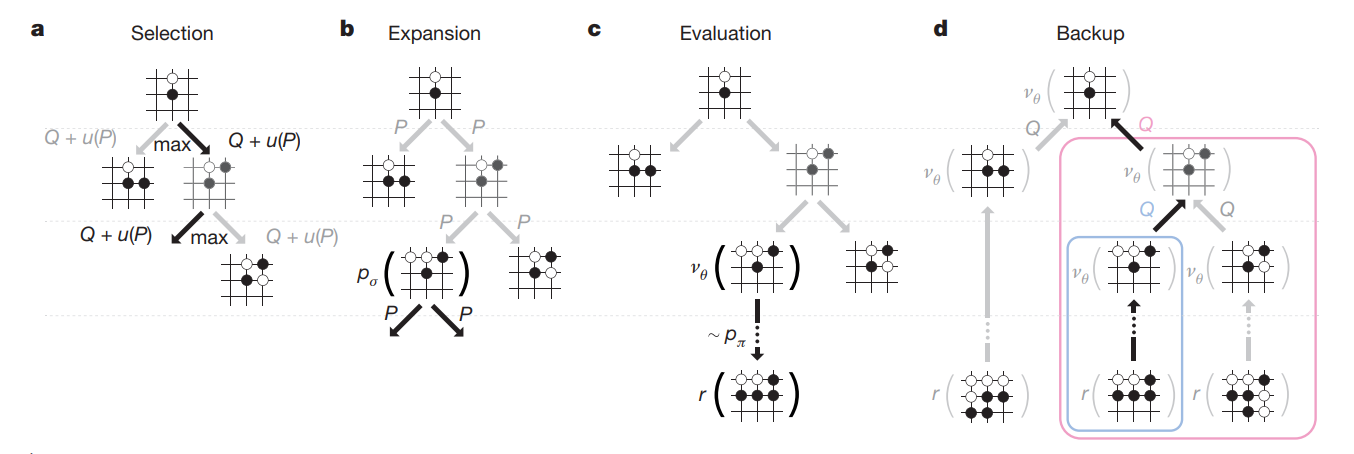
\includegraphics[width=10.5cm, height=3.8cm]{ressources/AlphaGo/MCTS_AlphaGo}
        \begin{block}{ Fonctions du MCTS }
            \begin{columns}[t]
                \begin{column}{0.45\textwidth}
                    Calcul de la valeur de l'action $a$ dans la position $s$.
                    $$Q(s,a) = \frac{1}{N(s,a)}\sum\limits_{i=1}^{n} 1_{s,a,i} V(s_L)$$

                \end{column}
                \begin{column}{0.45\textwidth}
                    Fonction bonus inversement proportionnelle aux visites du noeud.
                    $$u(s,a) \propto \frac{P(s,a)}{1+N(s,a)}$$
                \end{column}
            \end{columns}
        \end{block}
    \end{center}
\end{frame}

\begin{frame}{AlphaGo}{MCTS}
    \begin{center}
        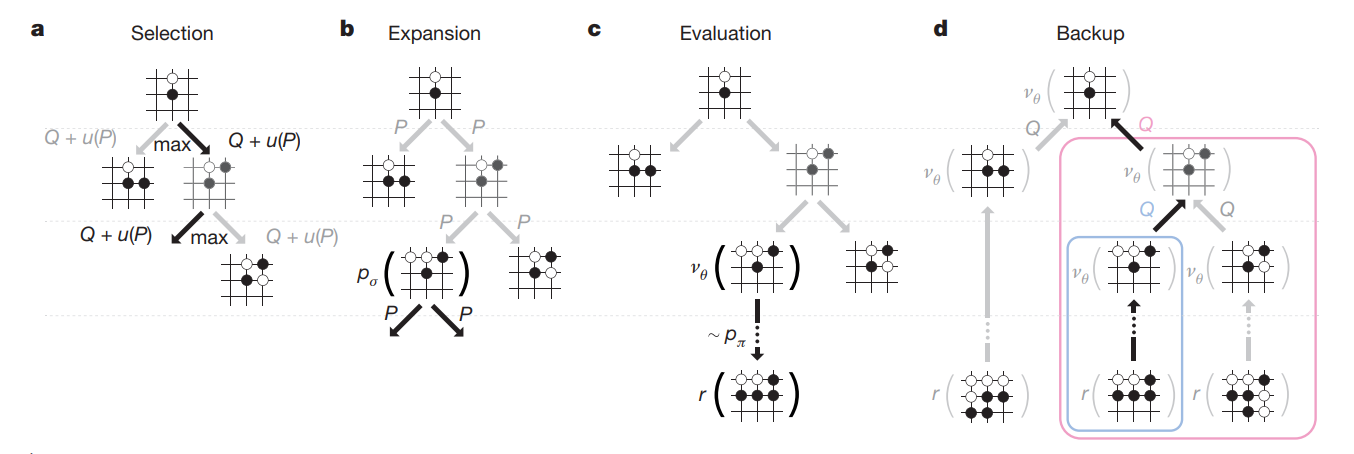
\includegraphics[width=10.5cm, height=3.8cm]{ressources/AlphaGo/MCTS_AlphaGo}
        \begin{block}{ Fonctions du MCTS }
            \begin{columns}[t]
                \begin{column}{0.45\textwidth}
                    Calcul de la valeur de l'action $a$ dans la position $s$, selon la politique $p_\sigma$:
                    $$P(s,a) = p_\sigma(a|s)$$

                \end{column}
                \begin{column}{0.45\textwidth}
                    Calcul du nombre de visites du noeud:
                    $$N (s,a) = \sum\limits_{i=1}^{n} 1_{s,a,i} $$
                \end{column}

            \end{columns}
        \end{block}

    \end{center}
\end{frame}

\begin{frame}{AlphaGo}{MCTS}
    \begin{center}
        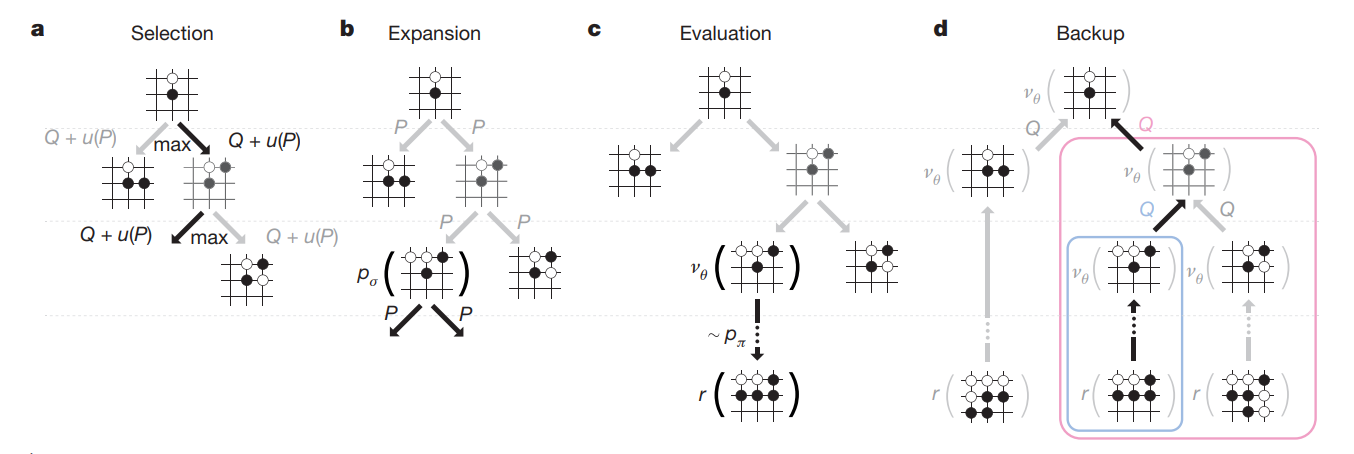
\includegraphics[width=10.5cm, height=3.8cm]{ressources/AlphaGo/MCTS_AlphaGo}
        \begin{block}{ Fonctions du MCTS }
            Valeur de la position $s_L$:
            $$V(s_L)=(1-\lambda)v_\theta(s_L) + \lambda z_L \mbox{, avec } \lambda \in [0,1]$$
        \end{block}
    \end{center}
\end{frame}

\begin{frame}{AlphaGo}{Résultats}
    \begin{columns}[t]
        \begin{column}{.4\textwidth}
            \vspace{-1.5cm}
            \begin{figure}
                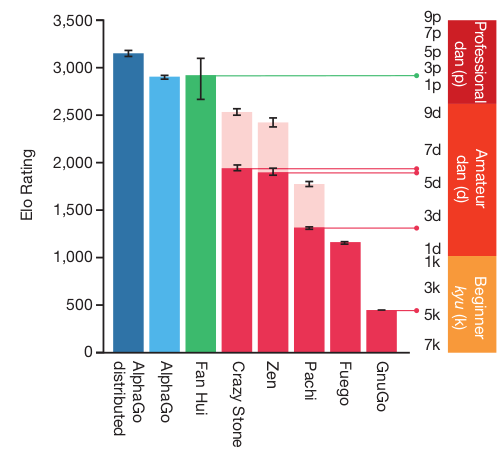
\includegraphics[scale=0.3]{ressources/AlphaGo/AlphaGovsShit.png}
                Elo de AlphaGo comparé à d'autres IA
            \end{figure}
        \end{column}
        \begin{column}{.4\textwidth}
            \begin{figure}
                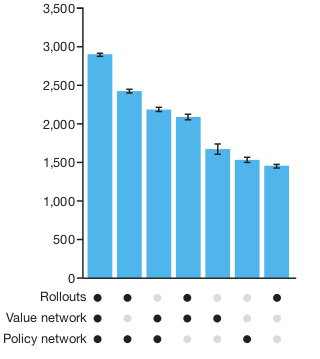
\includegraphics[scale=0.3]{ressources/AlphaGo/comparaison_different_models}
                \\
                Elo de AlphaGo selon les composants utilisés
            \end{figure}
        \end{column}
    \end{columns}
\end{frame}
